\documentclass[a4j,12pt,]{jarticle}
 \usepackage[dvipdfmx]{graphicx}
 \usepackage{float}
 \usepackage{siunitx} %%SI単位系用
 \usepackage{amssymb, amsmath}
 \usepackage{ascmac,here,txfonts,txfonts}
\usepackage{listings,jlisting}
\usepackage[dvipdfmx]{color}
\lstset{%
  language={Python},
  basicstyle={\small},%
  identifierstyle={\small},%
  commentstyle={\small\itshape\color[rgb]{0,0.5,0}},%
  keywordstyle={\small\bfseries\color[rgb]{0,0,1}},%
  ndkeywordstyle={\small},%
  stringstyle={\small\ttfamily\color[rgb]{1,0,1}},
  frame={tb},
  breaklines=true,
  columns=[l]{fullflexible},%
  numbers=left,%
  xrightmargin=0zw,%
  xleftmargin=3zw,%
  numberstyle={\scriptsize},%
  stepnumber=1,
  numbersep=1zw,%
  lineskip=-0.5ex%
}
\begin{document}

{\noindent\small 第5回報告書 \hfill\today}
\begin{center}
  {\Large 日射量の実測値と計算値の比較}
\end{center}
\begin{flushright}
  祖父江匠真 \\
\end{flushright}

\section{はじめに}
前回, 任意の緯度経度と日時から日射量を計算するプログラムを開発したので, リサイクル館から送信された太陽光発電の日射量のデータとプログラムによって計算された日射量を比較, 評価する.

\section{実測値データの取得}
リサイクル館から送信された太陽光発電データを保存しているElasticsearchサーバーから任意の日付におけるドキュメントを全て取得するプログラムをソースコード\ref{sc1}に示す.
なお, Elasticsearchサーバーには1日あたり約45000件のドキュメントが保存されていたため, ソースコード\ref{sc1}では, ScrollAPIを用いてドキュメントの取得を行っている.

\begin{lstlisting}[caption=Elasticsearchサーバーから任意の日付の環境データを取得するプログラム, label=sc1]
from elasticsearch import Elasticsearch
import pickle
import datetime
import os


def fetchDocsByDatetime(dt_crr, filePath):
    es = Elasticsearch("http://133.71.201.197:9200", http_auth=("takenaka", "takenaka"))

    indexName = "pcs_recyclekan"

    # すでにPickleファイルが存在するならElasticSearchから取得しない
    if os.path.isfile(filePath):
        return

    dt_next = dt_crr + datetime.timedelta(days=1)
    query = {
        "query": {
            "range": {
                "JPtime": {
                    "gte": f"{dt_crr.year}-{str(dt_crr.month).zfill(2)}-{str(dt_crr.day).zfill(2)}T00:00:00",
                    "lt": f"{dt_next.year}-{str(dt_next.month).zfill(2)}-{str(dt_next.day).zfill(2)}T00:00:00",
                },  # JST時間をUTC時間として登録しているのでUTC時間として検索する必要がある
            }
        }
    }

    num = 10
    s_time = "2m"
    data = es.search(
        index=indexName,
        scroll=s_time,
        body=query,
        size=num,
        request_timeout=150,
    )

    s_id = data["_scroll_id"]
    s_size = data["hits"]["total"]["value"]
    result = data["hits"]["hits"]
    while s_size > 0:
        data = es.scroll(scroll_id=s_id, scroll=s_time, request_timeout=150)
        s_id = data["_scroll_id"]
        s_size = len(data["hits"]["hits"])
        result.extend(data["hits"]["hits"])

    with open(filePath, "wb") as f:
        pickle.dump(result, f)

    # 内部接続を閉じる
    es.close()
\end{lstlisting}

\section{実測値と計算値をプロットする}
ソースコード\ref{sc1}によって取得したElasticsearchサーバーの日射量データと, 計算によって求めた日射量データをプロットしたものを図\ref{p1}に示す.
図\ref{p1}はElasticsearchサーバーから取得した2022年5月3日の日射量データと, 2022年5月3日のリサイクル館の緯度経度を入力として求めた日射量の計算値をプロットしている.
また, Elasticsearchサーバーから取得したドキュメント数は約45000件であったが全てをプロットするとPCがフリーズしてしまったので, 1分辺り1件にドキュメントを絞り込んでプロットしている.
更に, 実測値と計算値の最大値が等しくなるよう, 計算値の縦軸のスケールを実測値と計算値の比率を元に変更している.

\begin{figure}[H]
  \begin{center}
    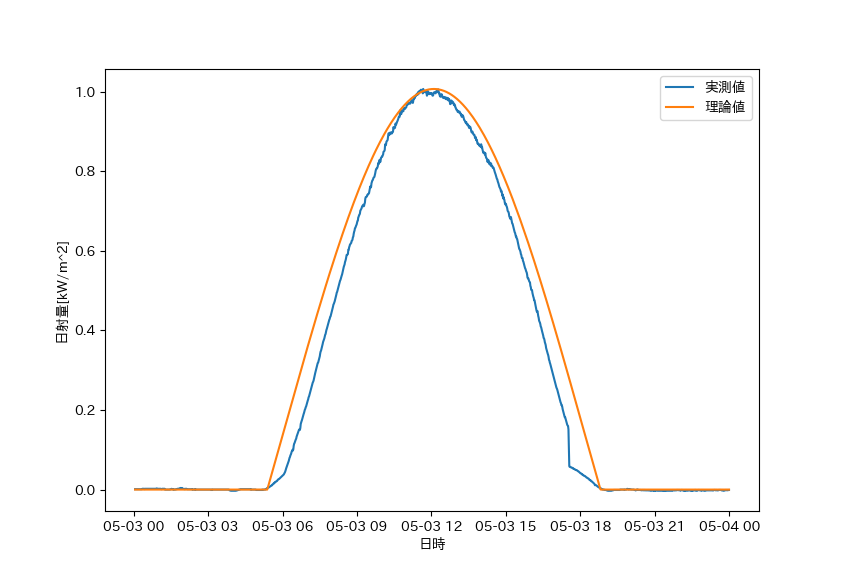
\includegraphics[width=160mm]{compare.png}
    \caption{2022年5月3日の日射量の実測値と計算値をプロットしたもの}
    \label{p1}
  \end{center}
\end{figure}

% 次に, 同時刻の実測値と計算値のペアについて, 計算値と同じ値を取る実測値と, ペアの実測値との時間差を各ペアごとに計算してプロットしたものを図\ref{p2}に示す.
次に, 計算値と同じ値を取る実測値の時刻と, 計算値の時刻の差を計算することで, 計算値を用いて時刻を予測した際の予測誤差を各計算値ごとに求めたものを図\ref{p2}に示す.
図\ref{p2}より, 計算によって求めた日射量による時刻の推定には最大で約59分の誤差が生じることが分かった.

\begin{figure}[H]
  \begin{center}
    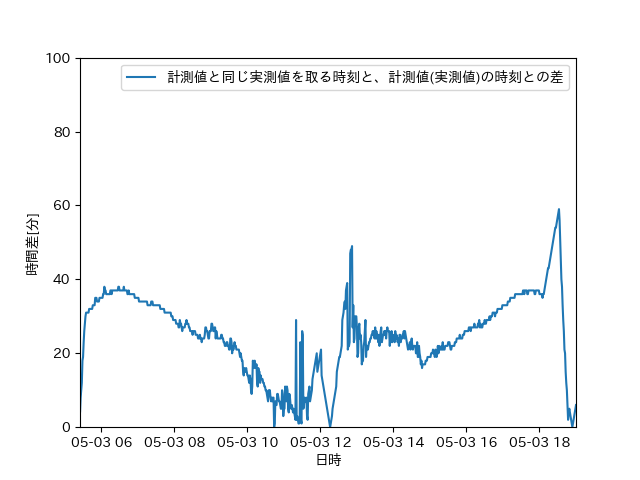
\includegraphics[width=160mm]{timeDiff.png}
    \caption{計測値と同じ実測値を取る時刻と、計測値の時刻との差}
    \label{p2}
  \end{center}
\end{figure}

\section{おわりに}
今回は, 実測した日射量のデータと計算によって求めた日射量を比較した.
計算値による時刻の推定に最大で約59分の誤差が生じていることが分かったので, 次回までに日射量の計算式を再検討する.

\begin{thebibliography}{5}
  \bibitem{1}祖父江匠真,"第4回報告書", Teams内,参照 May 30, 2022.
\end{thebibliography}

\end{document}